\subsection{Outros}


\subsubsection{Primeira letra em destaque}

Destacar a primeira letra de um texto.

\begin{figure}[!ht]
    \centering
    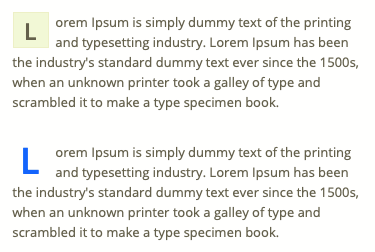
\includegraphics[scale=.5]{dropcaps}
    \caption{Primeira letra em destaque}\label{RS0001:fig:dropcaps}
\end{figure}

\begin{code}
    \inputminted[label=dropcaps.html]{html}{../RS0001/anexos/dropcaps.html}
    \caption{Exemplo de primeira letra em destaque}\label{RS0001:code:exemplo-dropcaps}
\end{code}


\subsubsection{Bloco de citação}

Bloco contendo uma citação, com nome do autor.

\begin{figure}[!ht]
    \centering
    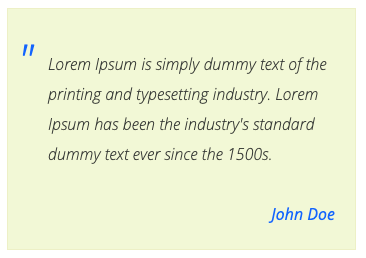
\includegraphics[scale=.5]{blockquote}
    \caption{Bloco de citação}\label{RS0001:fig:blockquote}
\end{figure}

\begin{code}
    \inputminted[label=blockquote.html]{html}{../RS0001/anexos/blockquote.html}
    \caption{Exemplo de citação}\label{RS0001:code:exemplo-blockquote}
\end{code}


\subsubsection{Listas}

Vários tipos diferentes de listas.

\begin{figure}[!ht]
    \centering
    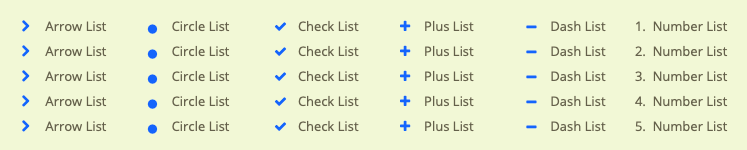
\includegraphics[scale=.5]{lists}
    \caption{Vários tipos de listas}\label{RS0001:fig:lists}
\end{figure}

\begin{code}
    \inputminted[label=lists.html]{html}{../RS0001/anexos/lists.html}
    \caption{Exemplos de listas}\label{RS0001:code:exemplo-lists}
\end{code}


\subsubsection{Tabelas}

Vários exemplos de tabelas.

\begin{figure}[!ht]
    \centering
    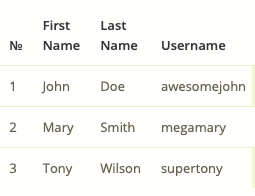
\includegraphics[scale=.5]{tables-1}
    \caption{Tabela simples}\label{RS0001:fig:tables-1}
\end{figure}

\begin{code}
    \inputminted[label=tables-1.html]{html}{../RS0001/anexos/tables-1.html}
    \caption{Exemplo de tabela simples}\label{RS0001:code:exemplo-tables}
\end{code}

\begin{figure}[!ht]
    \centering
    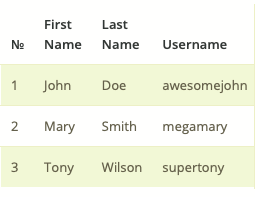
\includegraphics[scale=.5]{tables-2}
    \caption{Tabela com linhas de cores alternadas}\label{RS0001:fig:tables-2}
\end{figure}

\begin{code}
    \inputminted[label=tables-2.html]{html}{../RS0001/anexos/tables-2.html}
    \caption{Exemplo de tabela com linhas de cores alternadas}\label{RS0001:code:exemplo-tables-2}
\end{code}

\begin{figure}[!ht]
    \centering
    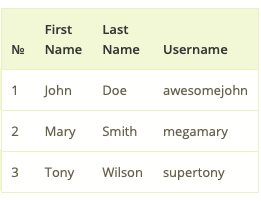
\includegraphics[scale=.5]{tables-3}
    \caption{Tabela com cabeçalho em destaque}\label{RS0001:fig:tables-3}
\end{figure}

\begin{code}
    \inputminted[label=tables-3.html]{html}{../RS0001/anexos/tables-3.html}
    \caption{Exemplo de tabela com cabeçalho em destaque}\label{RS0001:code:exemplo-tables-3}
\end{code}


\subsection{Organização do texto em colunas}

\subsubsection{Uma coluna}

\begin{figure}[!ht]
    \centering
    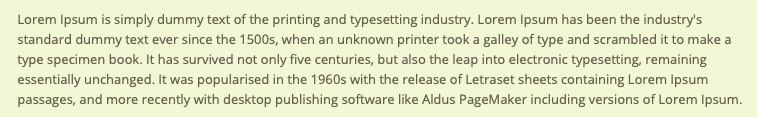
\includegraphics[scale=.5]{1-column}
    \caption{Uma coluna}\label{RS0001:fig:1-column}
\end{figure}

\begin{code}
    \inputminted[label=1-column.html]{html}{../RS0001/anexos/1-column.html}
    \caption{Exemplo de texto em uma coluna}\label{RS0001:code:exemplo-1-column}
\end{code}


\subsubsection{Duas colunas}

\begin{figure}[!ht]
    \centering
    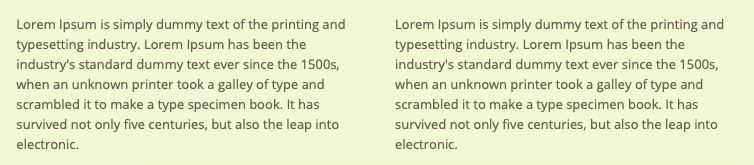
\includegraphics[scale=.5]{2-column}
    \caption{Duas colunas}\label{RS0001:fig:2-column}
\end{figure}

\begin{code}
    \inputminted[label=2-column.html]{html}{../RS0001/anexos/2-column.html}
    \caption{Exemplo de texto em duas colunas}\label{RS0001:code:exemplo-2-column}
\end{code}


\subsubsection{Três colunas}

\begin{figure}[!ht]
    \centering
    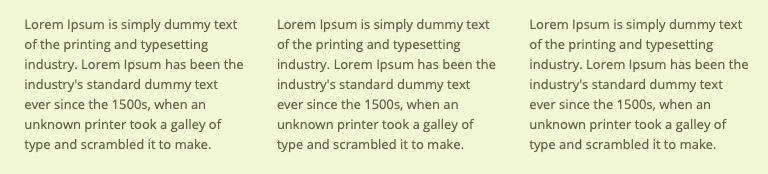
\includegraphics[scale=.5]{3-column}
    \caption{Três colunas}\label{RS0001:fig:3-column}
\end{figure}

\begin{code}
    \inputminted[label=3-column.html]{html}{../RS0001/anexos/3-column.html}
    \caption{Exemplo de texto em três colunas}\label{RS0001:code:exemplo-3-column}
\end{code}


\subsubsection{2/3 e 1/3 de espaço}

\begin{figure}[!ht]
    \centering
    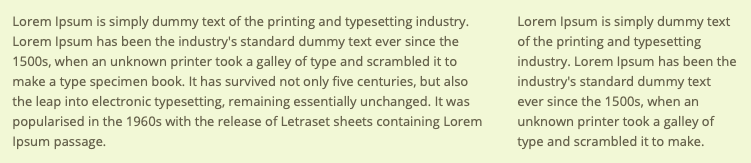
\includegraphics[scale=.5]{2-1-column}
    \caption{2/3 e 1/3 de espaço}\label{RS0001:fig:2-1-column}
\end{figure}

\begin{code}
    \inputminted[label=2-1-column.html]{html}{../RS0001/anexos/2-1-column.html}
    \caption{Exemplo de textos em 2/3 e 1/3 de espaço}\label{RS0001:code:exemplo-2-1-column}
\end{code}


\subsubsection{Quatro colunas}

\begin{figure}[!ht]
    \centering
    
\includegraphics[scale=.5]{4-column}
    \caption{Quatro colunas}\label{RS0001:fig:4-column}
\end{figure}

\begin{code}
    \inputminted[label=1-4-column.html]{html}{../RS0001/anexos/4-column.html}
    \caption{Exemplo de texto em 4 colunas}\label{RS0001:code:exemplo-4-column}
\end{code}


\subsubsection{3/4 e 1/4 de espaço}

\begin{figure}[!ht]
    \centering
    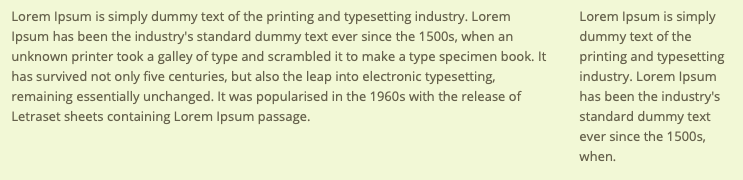
\includegraphics[scale=.5]{3-1-column}
    \caption{3/4 e 1/4 de espaço}\label{RS0001:fig:3-1-column}
\end{figure}

\begin{code}
    \inputminted[label=3-1-column.html]{html}{../RS0001/anexos/3-1-column.html}
    \caption{Exemplo de textos em 3/4 e 1/4 de espaço}\label{RS0001:code:exemplo-3-1-column}
\end{code}